\documentclass[a4paper]{article}

\usepackage{polski}
\usepackage[utf8]{inputenc}

\usepackage[export]{adjustbox}
\usepackage{scrextend}
\usepackage{amsfonts}
\usepackage{amsmath}
\usepackage{svg}


\usepackage{geometry}
\geometry{a4paper, left=15mm, top=30mm, right=15mm, bottom=20mm}

\usepackage{gensymb}
\usepackage{graphicx} 
\usepackage{isotope}
\usepackage{array}
\usepackage{float}
\usepackage{titlesec}
\usepackage{fancyhdr}
\usepackage{multirow}

\usepackage{hyperref}
\usepackage{sectsty}
\usepackage{enumitem}
\usepackage{listings}
\usepackage[labelformat=simple]{subcaption}
\usepackage{xcolor,colortbl}
\usepackage{animate}

\sectionfont{\normalfont\huge\sectionrule{0pt}{0pt}{-6pt}{1pt}}
\subsectionfont{\normalfont\LARGE}

\pagestyle{fancy}
\fancyhf{}
\fancyhead[LE,LO]{\Large Łukasz Kwinta}
\fancyhead[LE,RO]{\Large Laboratorium 3 - Triangulacja Wielokątów Monotonicznych}
\fancyfoot[CE,CO]{\Large\thepage}

\renewcommand{\footrulewidth}{1pt}
\renewcommand{\headrulewidth}{1pt}

\definecolor{Gray}{gray}{0.85}
\definecolor{LightGray}{gray}{0.95}

\newcolumntype{a}{>{\columncolor{Gray}}c}
\newcolumntype{b}{>{\columncolor{white}}c}

\hypersetup{
    colorlinks,
    citecolor=black,
    filecolor=black,
    linkcolor=black,
    urlcolor=black
}

\title{\fontsize{30pt}{30pt}\selectfont Laboratorium 3 \\ Triangulacja Wielokątów Monotonicznych}
\author{\fontsize{20pt}{20pt}\selectfont Łukasz Kwinta}
\date{}

\begin{document}
\maketitle
\Large
\vspace*{\fill}
\section{Dane Techniczne}
Procesor: AMD Ryzen 7 5700U\\
System operacyjny: Ubuntu 20.04 w środowisku WSL 2 na Windows 11 x64\\
Pamięć ram: 32 GB DDR4\\
\\
\\
Środowisko i język: Python 3.9 + Jupyter Notebook w środowisku Anaconda\\
Wykresy tworzyłem przy pomocy narzędzia przygotowanego przez KN Bit, 
do obliczeń numerycznych używałem biblioteki numpy.
 Dane przechowywałem w zmiennych typu float – typ danych o rozmiarze 64 bitów, 
 odpowiednik typu double w języku C.
\pagebreak
\section{Opis Realizacji Ćwiczenia}
Celem ćwiczenia była implementacja algorytmu obliczającego triangulację wielokątów 
monotonicznych.
    \subsection{Szczegóły techniczne}
    Do obliczeń używałem własnego wyznacznika 2x2 w postaci:
    \[
        \det{(a, b, c)} = (b.x - a.x)(c.y - b.y) - (b.y - a.y)(c.x - b.x)   
    \]
    a dokładność zera przyjąłem jako: $\varepsilon = 10^{-14}$
    \subsection{Sprawdzenie y-monotoniczności}
    Pierwszym krokiem była implementacja funkcji sprawdzającej y-monotoniczność wielokątów - 
    takich, które można podzielić na dwa łańcuchy w których kolejne wierzchołki wielokąta posortowane
    są rosnąco (jeden zgodnie ze wskazówkami zegara, drugi przeciwnie do wskazówek zegara). Przykładowy 
    wielokąt monotoniczny przedstawiłem na Rysunku \ref{fig:example_monotone}.
    \begin{figure}[H]
        \centering
        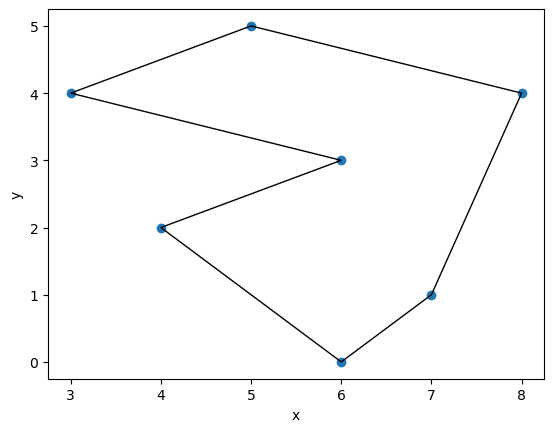
\includegraphics{przykladowy_y_monotoniczny.png}
        \caption{Przykładowy wielokąt y-monotoniczny}
        \label{fig:example_monotone}
    \end{figure}
    \noindent Sprawdzenia dokonałem przeglądając wierzchołki od takiego z najmniejszą współrzędną y
    w kierunku przeciwnym do kierunku wskazówek zegara i sprawdzam czy kolejne współrzędne rosną,
    a następnie po jednym punkcie zmiany monotoniczności maleją.

    \subsection{Klasyfikacja wierzchołków}
    Następną częścią ćwiczenia było zaklasyfikowanie różnych typów wierzchołków na następujące
    typy:
    \begin{itemize}
        \item Początkowe - oznaczone kolorem zielonym
        \item Końcowe - oznaczone kolorem czerwonym
        \item Dzielące - oznaczone kolorem cyjan
        \item Łączące - oznaczone kolorem niebieskim
        \item Prawidłowe - oznaczone kolorem brązowym 
    \end{itemize} 
    \noindent Na Rysunku \ref{fig:example_vertex_colors} przedstawiam przykładowy wynik klasyfikacji
    wierzchołków wielokąta.
    \begin{figure}[H]
        \centering
        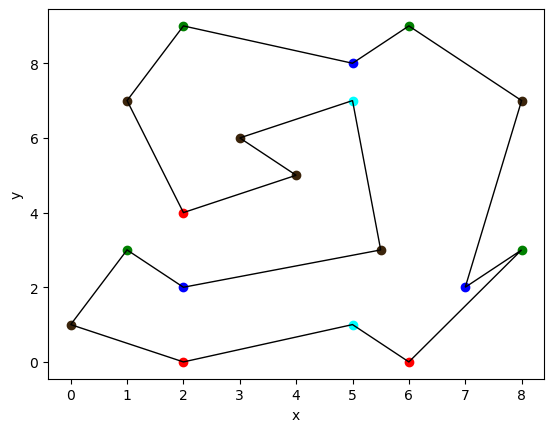
\includegraphics{przykladowa_klasyfikacja.png}
        \caption{Przykładowa klasyfikacja wierzchołków}
        \label{fig:example_vertex_colors}
    \end{figure}
    \noindent Taka klasyfikacja pozwala na podzielenie dowolnego wielokąta na wielokąty y-monotoniczne w
    celu triangulacji mniejszych części wielokąta prostą metodą. Powyższą metodą można też sprawdzić 
    monotoniczność wielokąta - wielokąt monotoniczny zawierać będzie tylko wierzchołki prawidłowe oraz dokładnie
    jeden początkowy i jeden końcowy, lecz z pewnością jest to mniej optymalny sposób niż poprzednia metoda. Do 
    sprawdzenia kąta wewnętrznego używałem wyznacznika 3 kolejnych punktów wielokąta.

\section{Triangulacja wielokąta y-monotonicznego}
    \subsection{Opis działania algorytmu}
    Ostatnim i docelowym elementem ćwiczenia była implementacja algorytmu tworzącego triangulację wielokąta
    y-monotonicznego. Wielokąt przechowywałem jako listę kolejnych wierzchołków w kolejności przeciwnej
    do kierunku wskazówek zegara. Do posortowania punktów względem kierunku monotoniczności użyłem funkcji 
    sortującej wbudowanej w listy języka Python z kluczem jako współrzędna y punktu. Zastosowałem metodę
    sortowania pośredniego przy pomocy tablicy indeksów pośrednich aby nie stracić informacji o początkowym 
    ułożeniu punktów w celu łatwego sprawdzania sąsiedztwa punktów.\\
    Aby ułatwić sprawdzanie czy nie dodaję takich samych przekątnych użyłem zbioru \verb|set()|, opartego o 
    hash-table zapewniającego dodawanie elementów w stałym czasie.\\
    Do określania czy sprawdzana przekątna znajduje się w czy poza wielokątem użyłem sprawdzenia odpowiedniego znaku
    wyznacznika punktów dla danego łańcucha.\\
    Algorytm w postaci listy kroków przedstawia się następująco:
    \begin{enumerate}
        \item Przypisanie punktom przynależności do łańcucha
        \item Posortowanie punktów wzdłuż kierunku monotoniczności
        \item Włożenie dwóch pierwszych wierzchołków na stos
        \item Sprawdzenie czy wierzchołek należy do tego samego łańcucha co wierzchołek na 
        szczycie stosu
        \begin{enumerate}
            \item Jeśli nie to możemy dodać przekątne do wszystkich wierzchołków na stosie, a nastepnie
            na stos trafiają dwa ostatnio rozważane wierzchołki
            \item Jeśli tak to badamy kolejne trójkąty składające się z przedostatniego i ostatniego wierzchołka
            ze stosu oraz badanego punktu:
            \begin{enumerate}
                \item Jeśli trójkąt należy do wielokąta, to dodajemy przekątną i rozważamy kolejny trójkąt
                \item Jeśli nie to rozważane wierzchołki dodajemy na stos
            \end{enumerate}
        \end{enumerate}
    \end{enumerate}
    \noindent Dzięki zastosowaniu sortowania pośredniego oraz użyciu zbioru do przechowywania listy przekątnych,
    algorytm ma złożoność $\mathcal{O} (n \log n)$ wynikającą z sortowania wierzchołków.\\
    Jako wynik algorytm zwraca krotki z indeksami wierzchołków między którymi znajduje się przekątna.
    \begin{figure}[H]
        \centering
        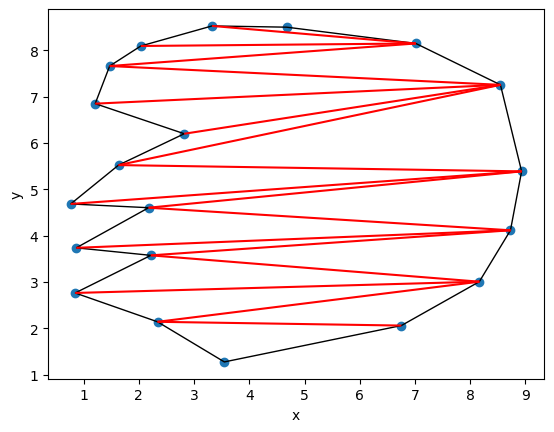
\includegraphics{przykladowa_triangulacja.png}
        \caption{Przykładowy wynik działania algorytmu}
        \label{fig:example_triangulation}
    \end{figure}
    
    \pagebreak
    \subsection{Wizualizacja działania algorytmu}
    Dokonałem modyfikacji algorytmu aby możliwa była wizualizacja kolejnych kroków działania algorytmy, 
    poniżej przedstawiam animację. \textbf{\textit{Uwaga! Animacja może nie działać w każdym
    programie do plików PDF, została przetestowana w programie Adobe Acrobat gdzie działa.
    W razie gdyby animacja nie działała będzie wyświetlona jedna klatka animacji. Samą 
    animację można znaleźć w notebooku z rozwiązaniem zadania.}}
    \begin{figure}[H]
        \centering
        \animategraphics[width=.9\textwidth, loop, autoplay, poster=30]{5}
        {animation_example/animation_example-}{0}{71}
        \caption{Animacja działania algorytmu na przykładowym wielokącie}
        \label{fig:animation_of_triangulation}
    \end{figure}
    

    \pagebreak
\section{Wielokąty testowe}
    \subsection{Wybór wielokątów testowych}    
    Poza testami algorytmu przygotowanymi przez KN Bit przygotowałem samemu 4 testowe wielokąty,
    przy pomocy zmodyfikowanego programu pozwalającemu na zadanie kolejnych punktów za pomocą myszki.
    Jako, że z oczywistych powodów nie mogłem testować algorytmu na dużych zbiorach danych 
    to postanowiłem zadać wielokąty o bardzo dużych współrzędnych i bardzo małych współrzędnych
    gdyż w takich przypadkach dokładność liczb zmiennoprzecinkowych gra istotną rolę i mogłyby 
    wystąpić błędy sugerujące dobranie złej dokładności zera. Jeśli chodzi o ułożenie punktów
    to zdecydowałem się na przetestowanie wielokątów z prostymi odcinkami i takich z 
    bokami w "zygzak". Wybrałem takie ułożone empirycznie na podstawie doświadczeń z 
    testami przygotowanymi przez KN Bit.\\\\
    Po analizie wyników algorytmu stwierdzam, że wyniki działania algorytmu są poprawne. \\\\
    W notebooku można też obejrzeć wizualizację działania algorytmu (animację).
    \pagebreak
    \subsection{Wielokąt A}
    Pierwszy wielokąt to taki którego współrzędne są rzędu $10^{13}$ i zawiera wspomniane wcześniej
    zygzaki na bokach.
    \begin{figure}[H]
        \centering
        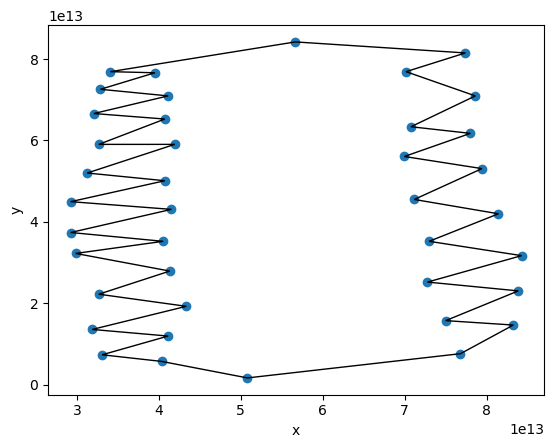
\includegraphics[width=.65\textwidth]{test_a_poly.png}
        \caption{Wizualizacja wielokąta testowego A}
        \label{fig:test_a_poly}
    \end{figure}
    \begin{figure}[H]
        \centering
        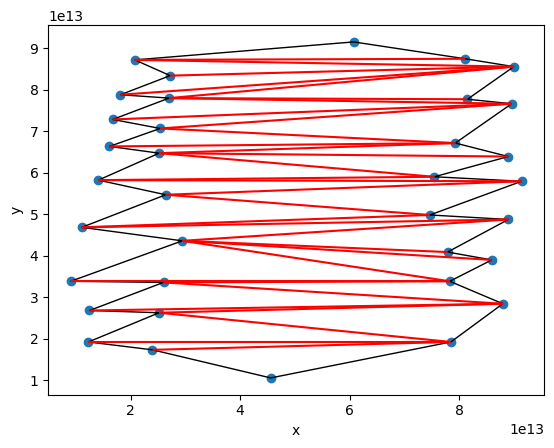
\includegraphics[width=.65\textwidth]{test_a_tri.png}
        \caption{Triangulacja wielokąta A}
        \label{fig:test_a_tri}
    \end{figure}

    \subsection{Wielokąt B}
    Kolejny wielokąt to taki którego współrzędne są rzędu $10^{13}$ i zawiera wspomniane wcześniej
    linie proste
    \begin{figure}[H]
        \centering
        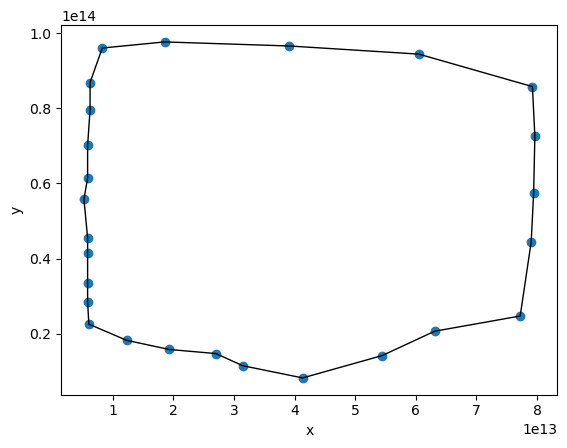
\includegraphics[width=.65\textwidth]{test_b_poly.png}
        \caption{Wizualizacja wielokąta testowego B}
        \label{fig:test_b_poly}
    \end{figure}
    \begin{figure}[H]
        \centering
        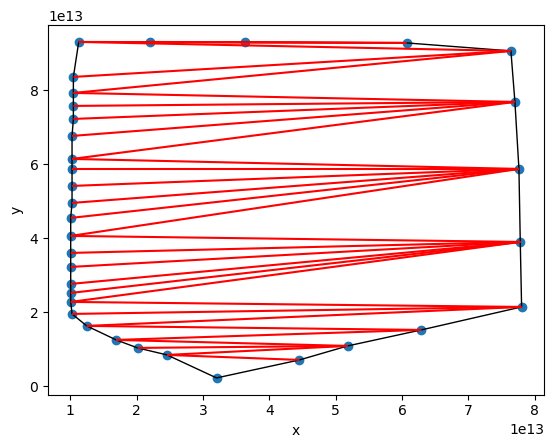
\includegraphics[width=.65\textwidth]{test_b_tri.png}
        \caption{Triangulacja wielokąta B}
        \label{fig:test_b_tri}
    \end{figure}

    \subsection{Wielokąt C}
    Pierwszy wielokąt to taki którego współrzędne są rzędu $10^{-15}$ i zawiera wspomniane wcześniej
    zygzaki na bokach.
    \begin{figure}[H]
        \centering
        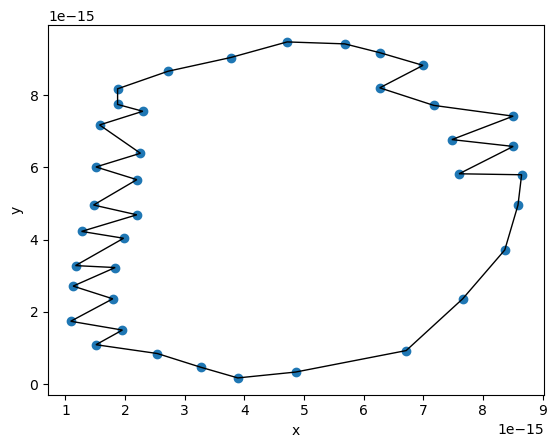
\includegraphics[width=.65\textwidth]{test_c_poly.png}
        \caption{Wizualizacja wielokąta testowego C}
        \label{fig:test_c_poly}
    \end{figure}
    \begin{figure}[H]
        \centering
        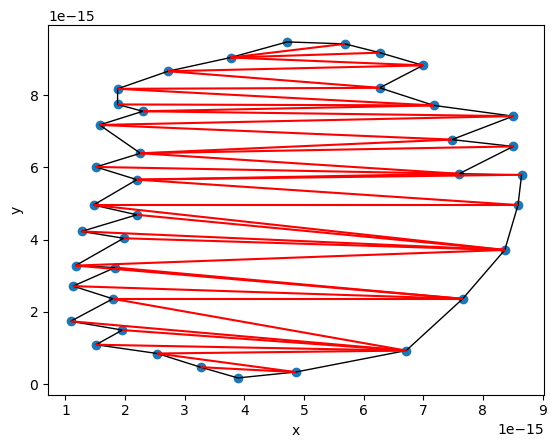
\includegraphics[width=.65\textwidth]{test_c_tri.png}
        \caption{Triangulacja wielokąta C}
        \label{fig:test_c_tri}
    \end{figure}

    \subsection{Wielokąt D}
    Kolejny wielokąt to taki którego współrzędne są rzędu $10^{-15}$ i zawiera wspomniane wcześniej
    linie proste
    \begin{figure}[H]
        \centering
        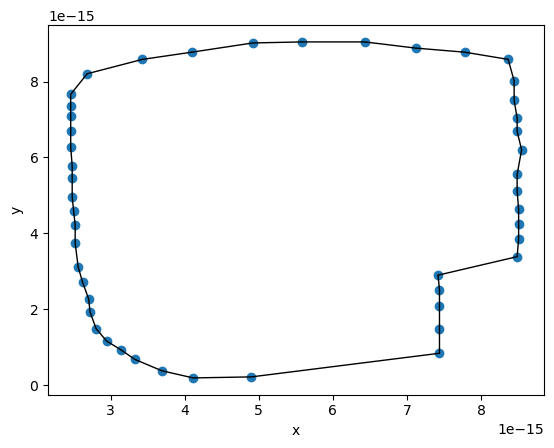
\includegraphics[width=.65\textwidth]{test_d_poly.png}
        \caption{Wizualizacja wielokąta testowego D}
        \label{fig:test_d_poly}
    \end{figure}
    \begin{figure}[H]
        \centering
        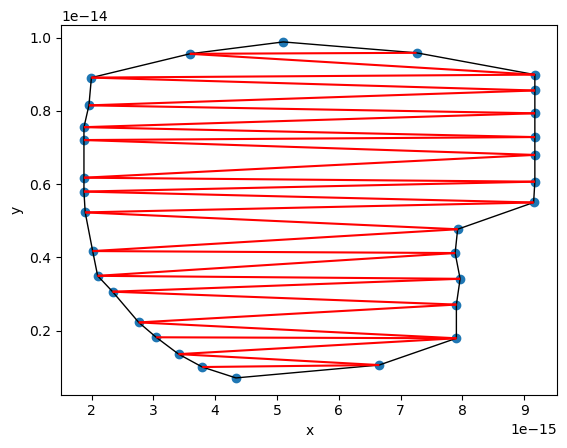
\includegraphics[width=.65\textwidth]{test_d_tri.png}
        \caption{Triangulacja wielokąta D}
        \label{fig:test_d_tri}
    \end{figure}
    
    

\section{Wnioski}
Na podstawie testów przygotowanych przez KN Bit jak i moich własnych przypadków testowych
można stwierdzić, że przedstawione algorytmu są zaimplementowane w prawidłowy sposób i 
dają prawidłowe wyniki. Najprawdopodobniej istnieją przypadki w których przyjęta dokładność
zera sprawiłaby, że algorytm nie będzie działał dokładnie lecz nie udało mi się wygenerować
takiego przypadku.

\end{document}